\documentclass[titlepage]{article}
\usepackage[tc]{titlepic}
\usepackage{graphicx}
\usepackage[top=25mm, bottom=25mm, left=27mm, right=27mm]{geometry}
\usepackage{caption}
\usepackage{listings}
\usepackage{lstlangarm}
\usepackage{tabu}
\usepackage{wrapfig}



\date{}
\author{Ali Bahadır Bulut\\ \#041602017  \and Alp
	Gokcek \\ \#041701014 \and Erdal Sidal Dogan \\ \#041702023}
\title{
\includegraphics[width=0.6\textwidth]{../images/logo_en_color.png}\\ 
\vspace{5em}
EE306 - Microprocessors\\
\vspace{2em}
\textbf{Term Project \linebreak Sliding Text
}\\
\vspace{1.5em}
June 8, 2020}

\begin{document}
	\maketitle
	\section{Project Description}
	2-3 cümlelik abstract/description (0-1): açıklayıcı, net olmalı.
	Lorem ipsum dolor sit amet, consectetur adipiscing elit. Integer at lectus est. Etiam pellentesque, dui eget tempor suscipit, turpis dui pharetra sapien, vel molestie enim felis ac est. Aliquam erat volutpat. Duis eget dictum lacus, nec luctus magna. Sed et cursus erat. Vivamus lobortis sollicitudin fringilla. In tincidunt mi arcu, quis suscipit metus hendrerit vitae. Sed ut libero sit amet orci pretium fermentum sit amet eu augue. Vivamus lobortis ante ut nunc porta posuere. Quisque vel leo a dui ultrices imperdiet.\\
	
	Our design supports the characters provided in Figure \ref{supported_chars}.\\
	
	\begin{figure}[h]
		\centering
		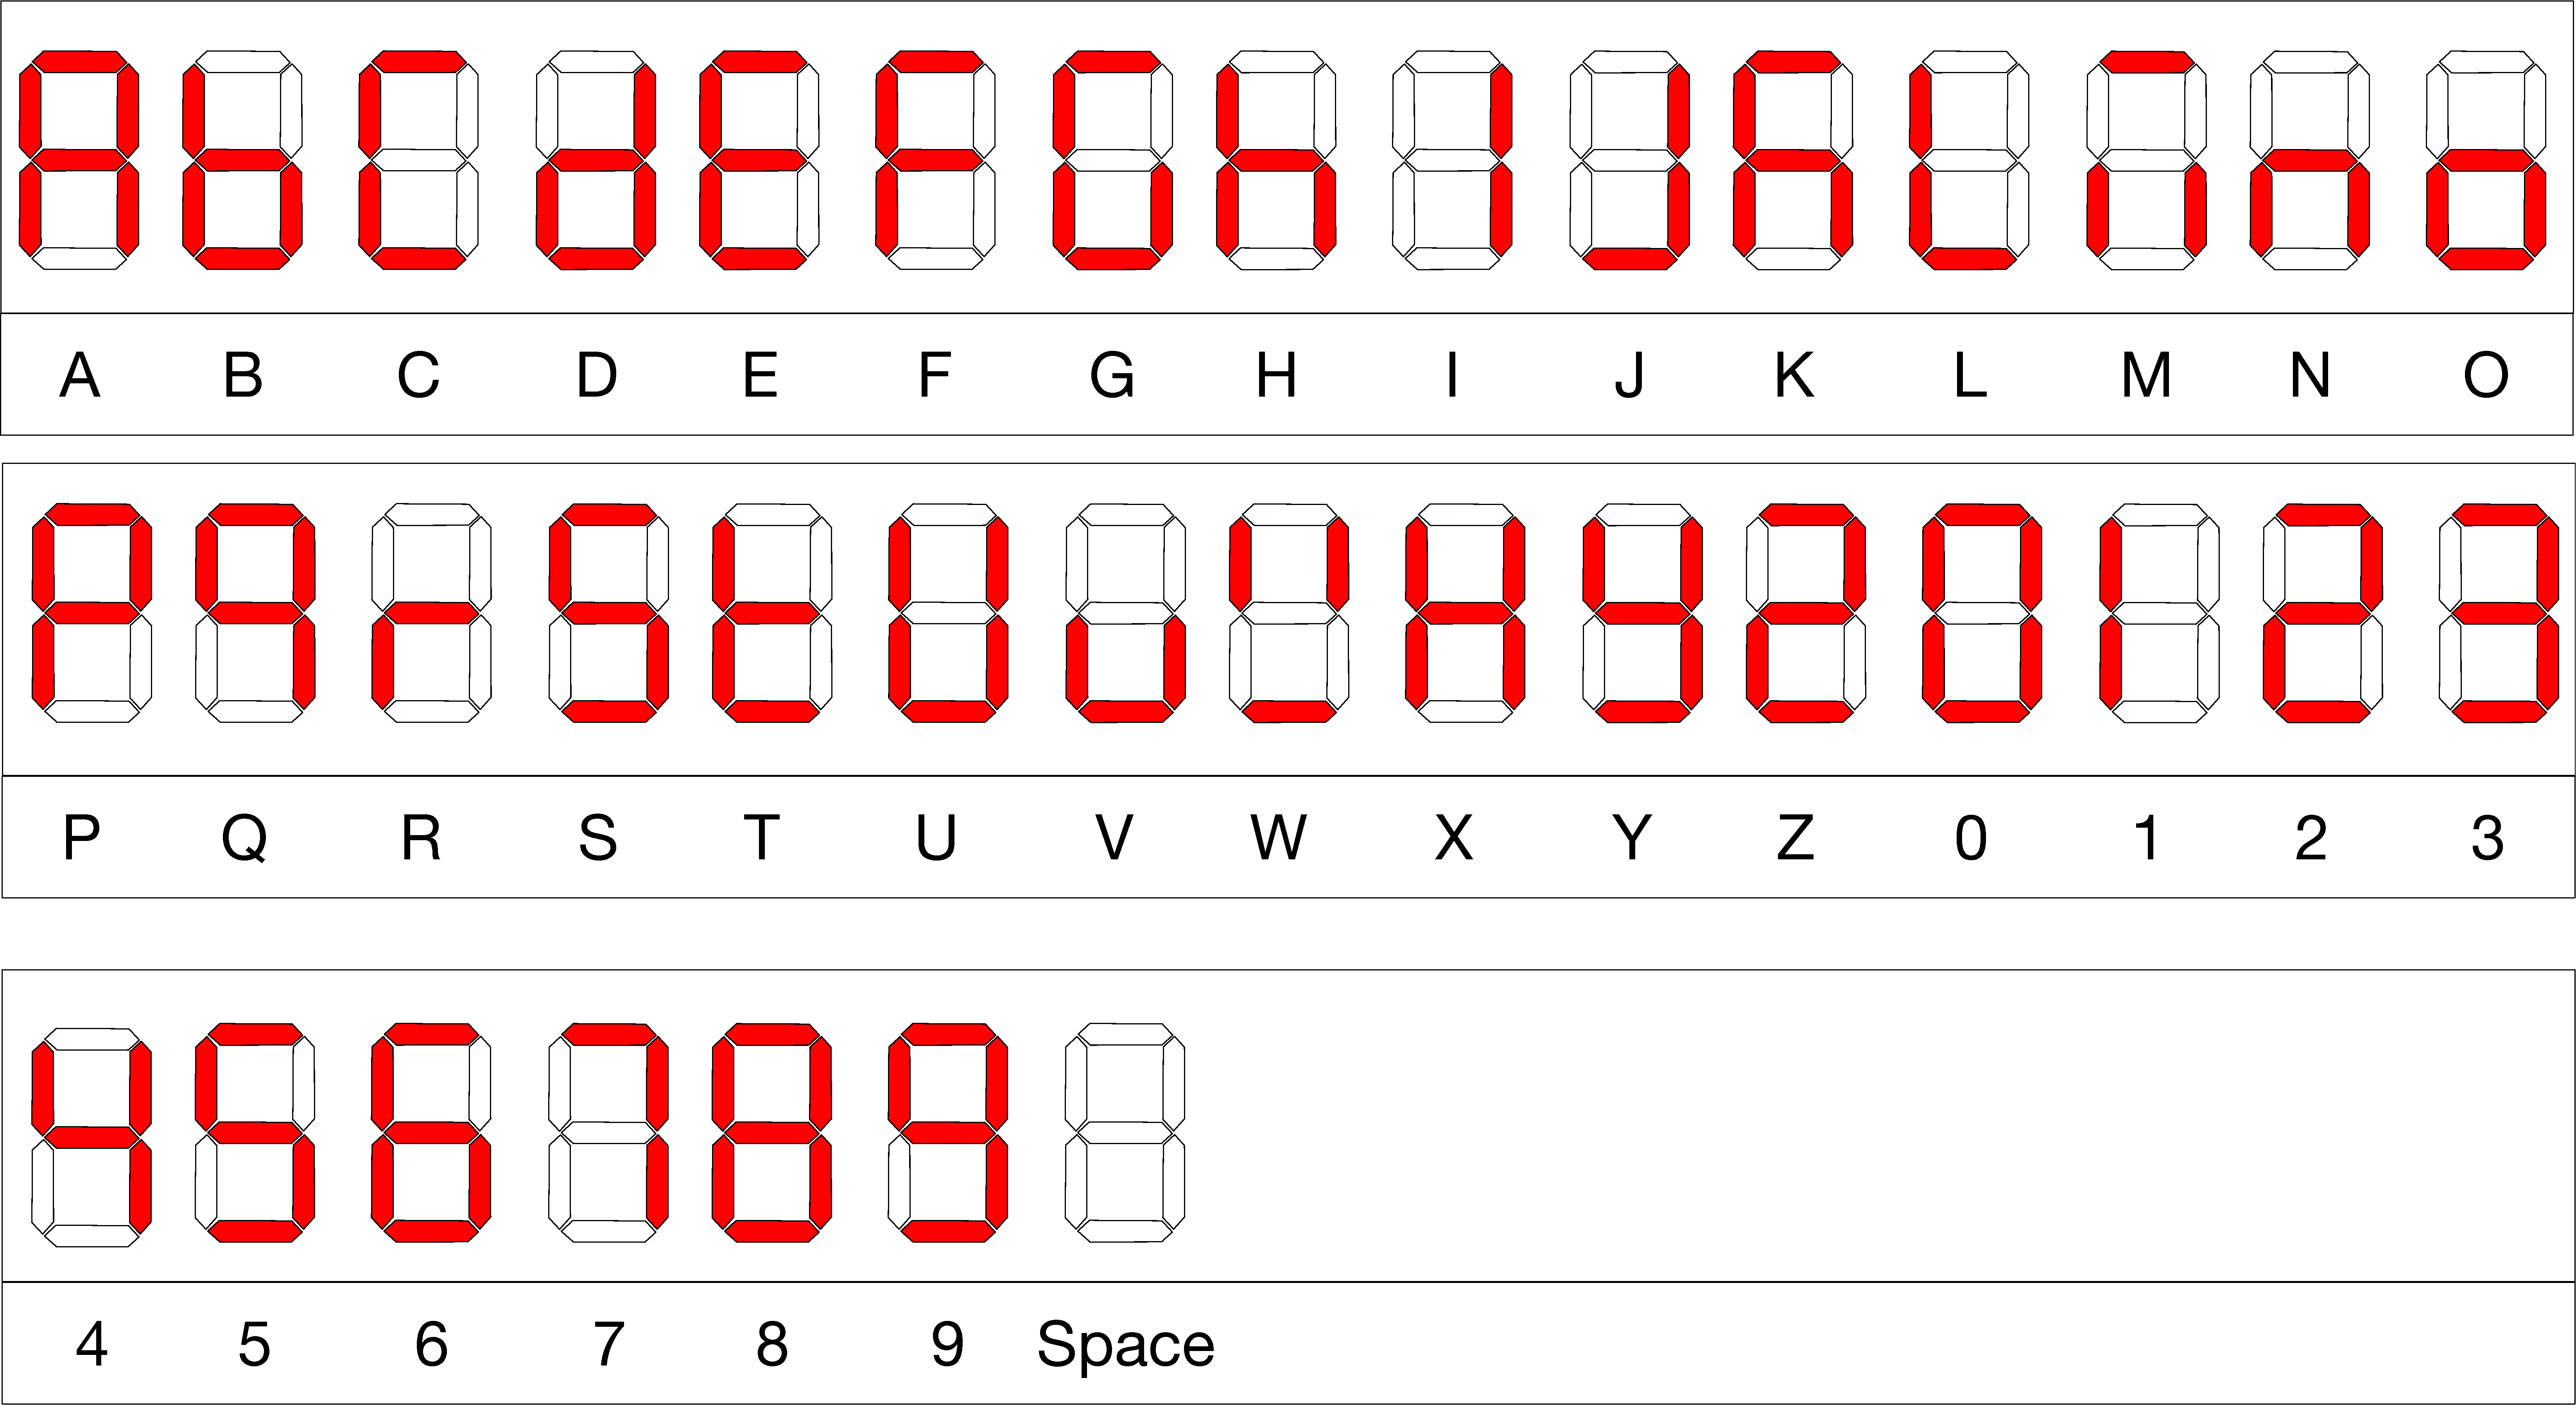
\includegraphics[scale=.1]{../images/supported_chars.pdf}
		\caption{Sample output on 7-segment displays for input "EE306 Fun"}
		\label{supported_chars}
	\end{figure}
	\section{Sample Output}
	\begin{figure}[h!]
		\centering
		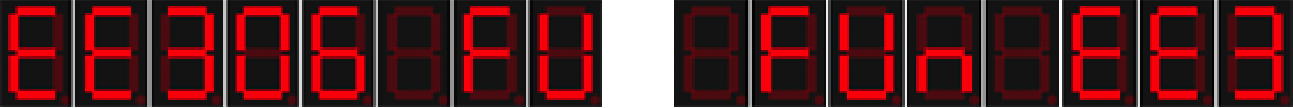
\includegraphics[scale=.45]{../images/fig1.png}
		\caption{Sample output on 7-segment displays for input "EE306 Fun"}
	\end{figure}

	\begin{figure}[h!]
		\centering
		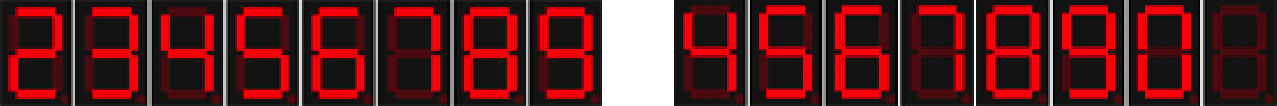
\includegraphics[scale=.45]{../images/fig2.png}
		\caption{Sample output on 7-segment displays for input "1234567890"}
	\end{figure}
	
	\begin{figure}[h!]
		\centering
		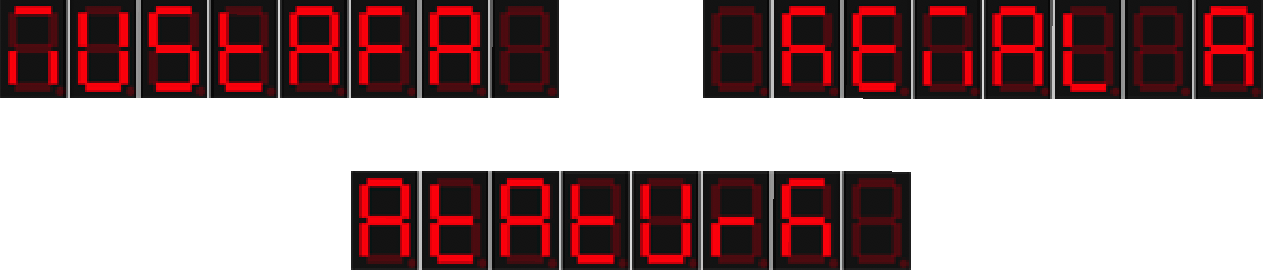
\includegraphics[scale=.45]{../images/fig3.png}
		\caption{Sample output on 7-segment displays for input "Mustafa Kemal Ataturk"}
	\end{figure}
	\section{Source Code}
	\lstinputlisting[language={[ARM]Assembler}, frame=single, basicstyle=\ttfamily, breaklines=true, showspaces=false, showstringspaces=false, caption=Source code of our sliding text project]{../source_codes/final_code.s} \label{source_code}
	\newpage
	\section{Flowcharts}
	\subsection{MAIN}
	After the initialization, the program starts executing the \textit{Main} subroutine. It consists of chaining other subroutines sequentially such as  \textit{SET\_WORD}, \textit{CHECK\_PAUSE}, \textit{SET\_SPEED}, \textit{PRINT\_STRING}.
	
	\begin{figure}[h]
		\centering
		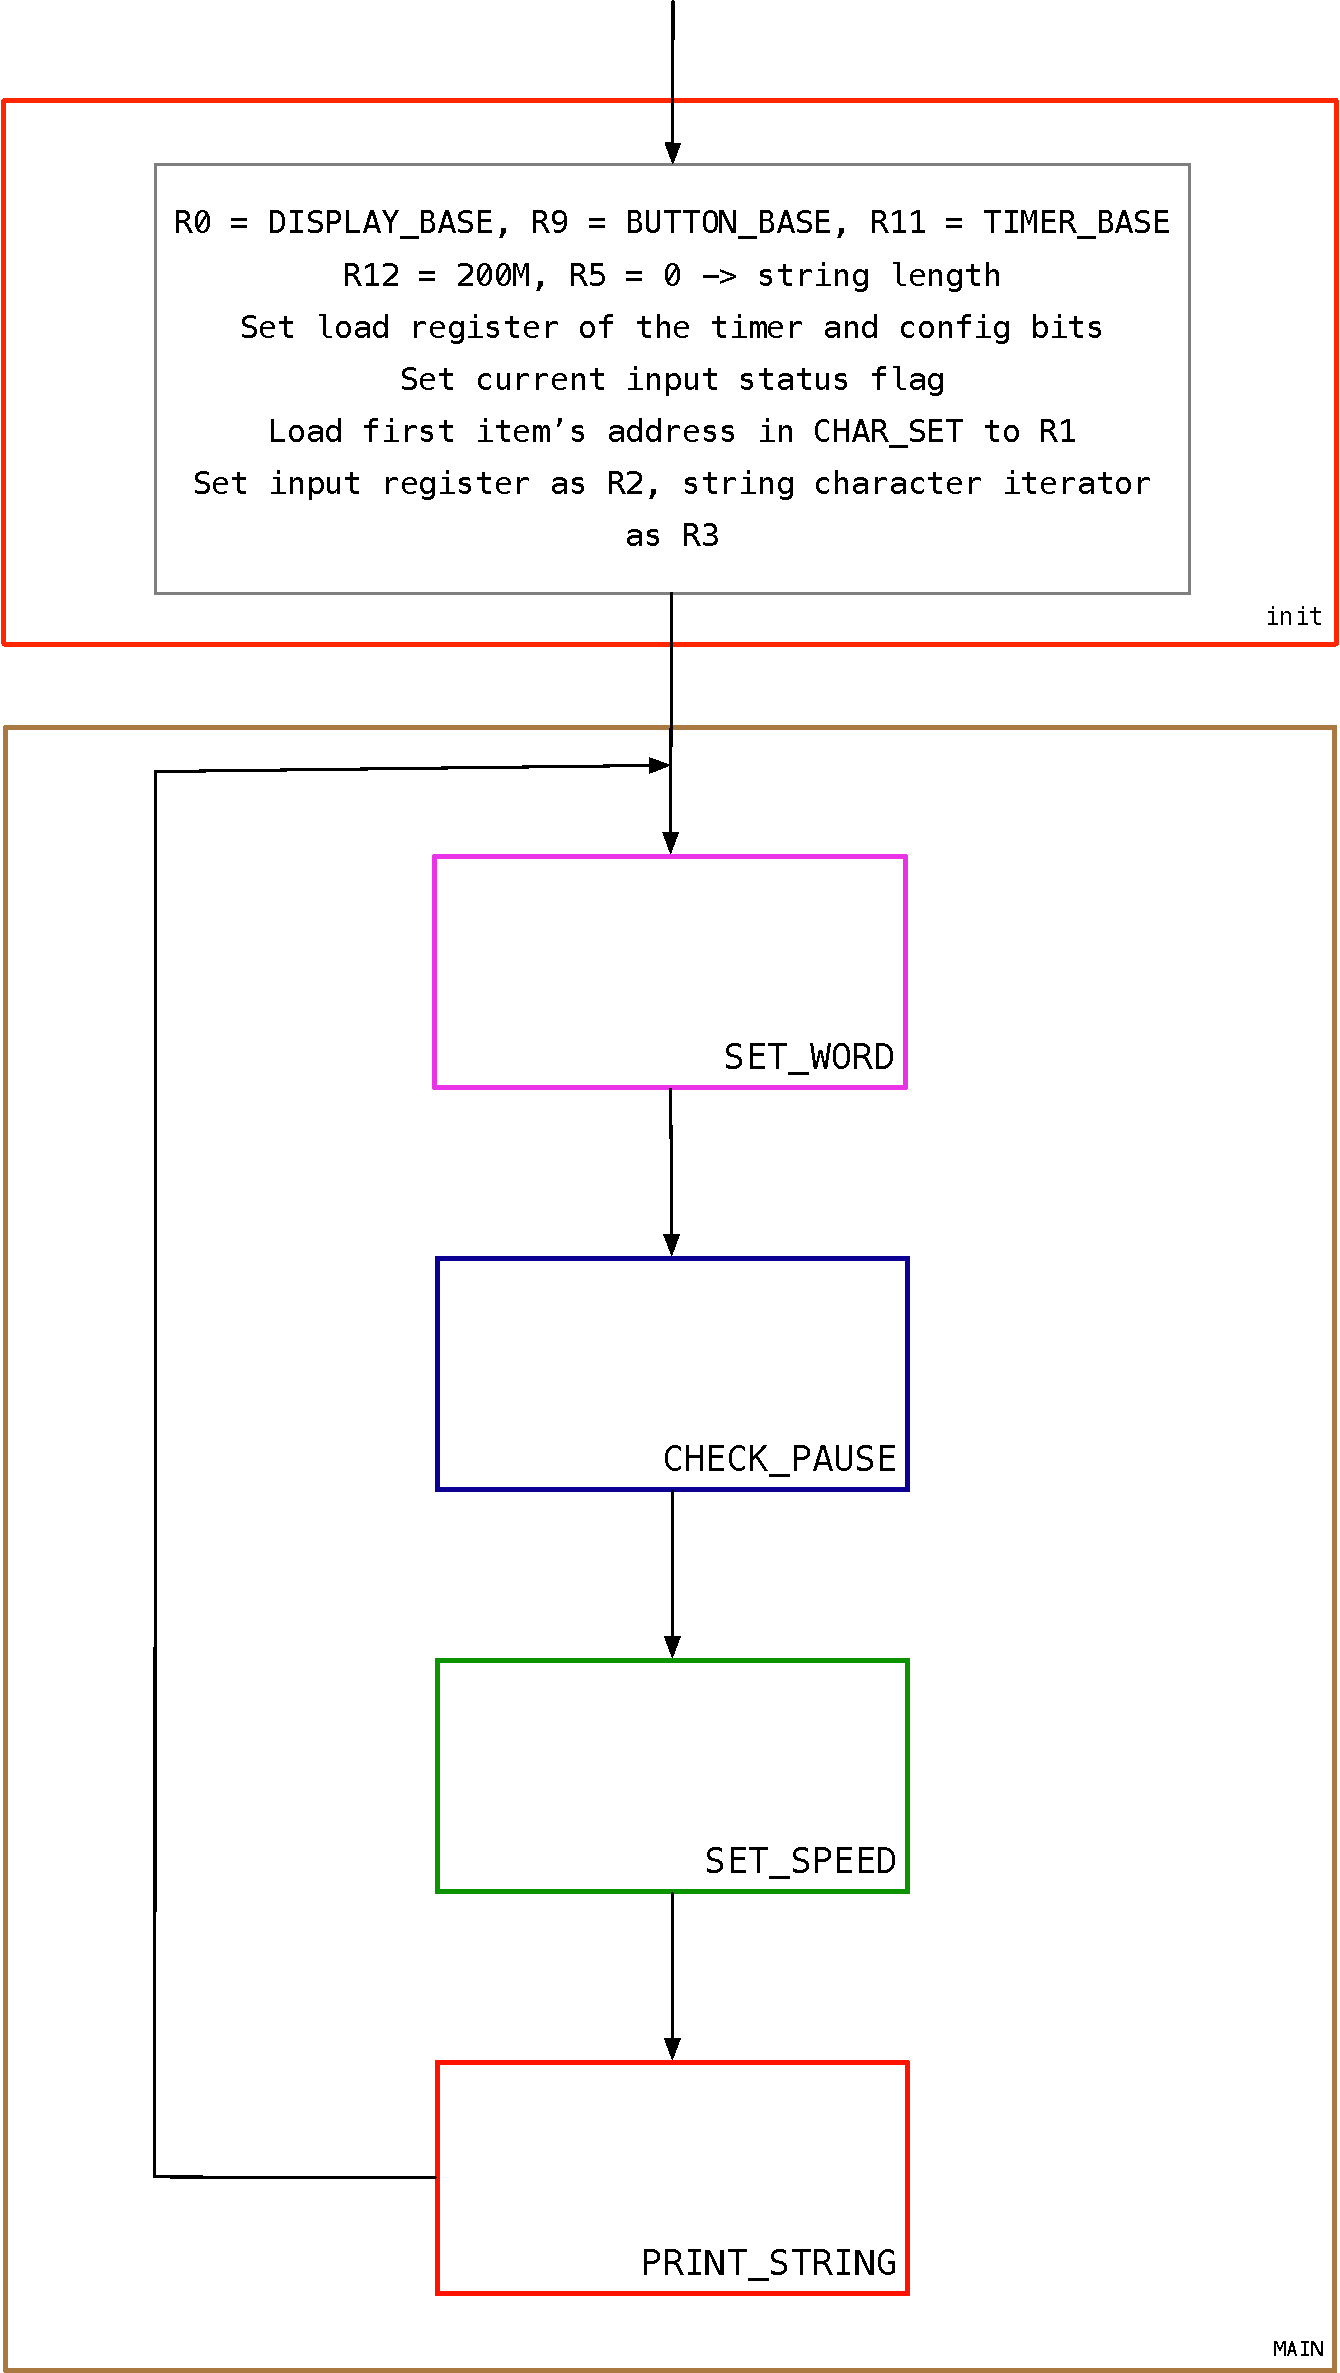
\includegraphics[scale=.3]{../images/main.pdf}
		\caption{Flowchart of Main Loop}
	\end{figure}
 	\newpage
	\subsection{SET\_WORD}
	The program supports multiple words. Selection is being made by the 'Switch' input. The subroutine \textit{SET\_WORD} is responsible for choosing the correct word according to the input.
	\begin{figure}[h]
		\centering
		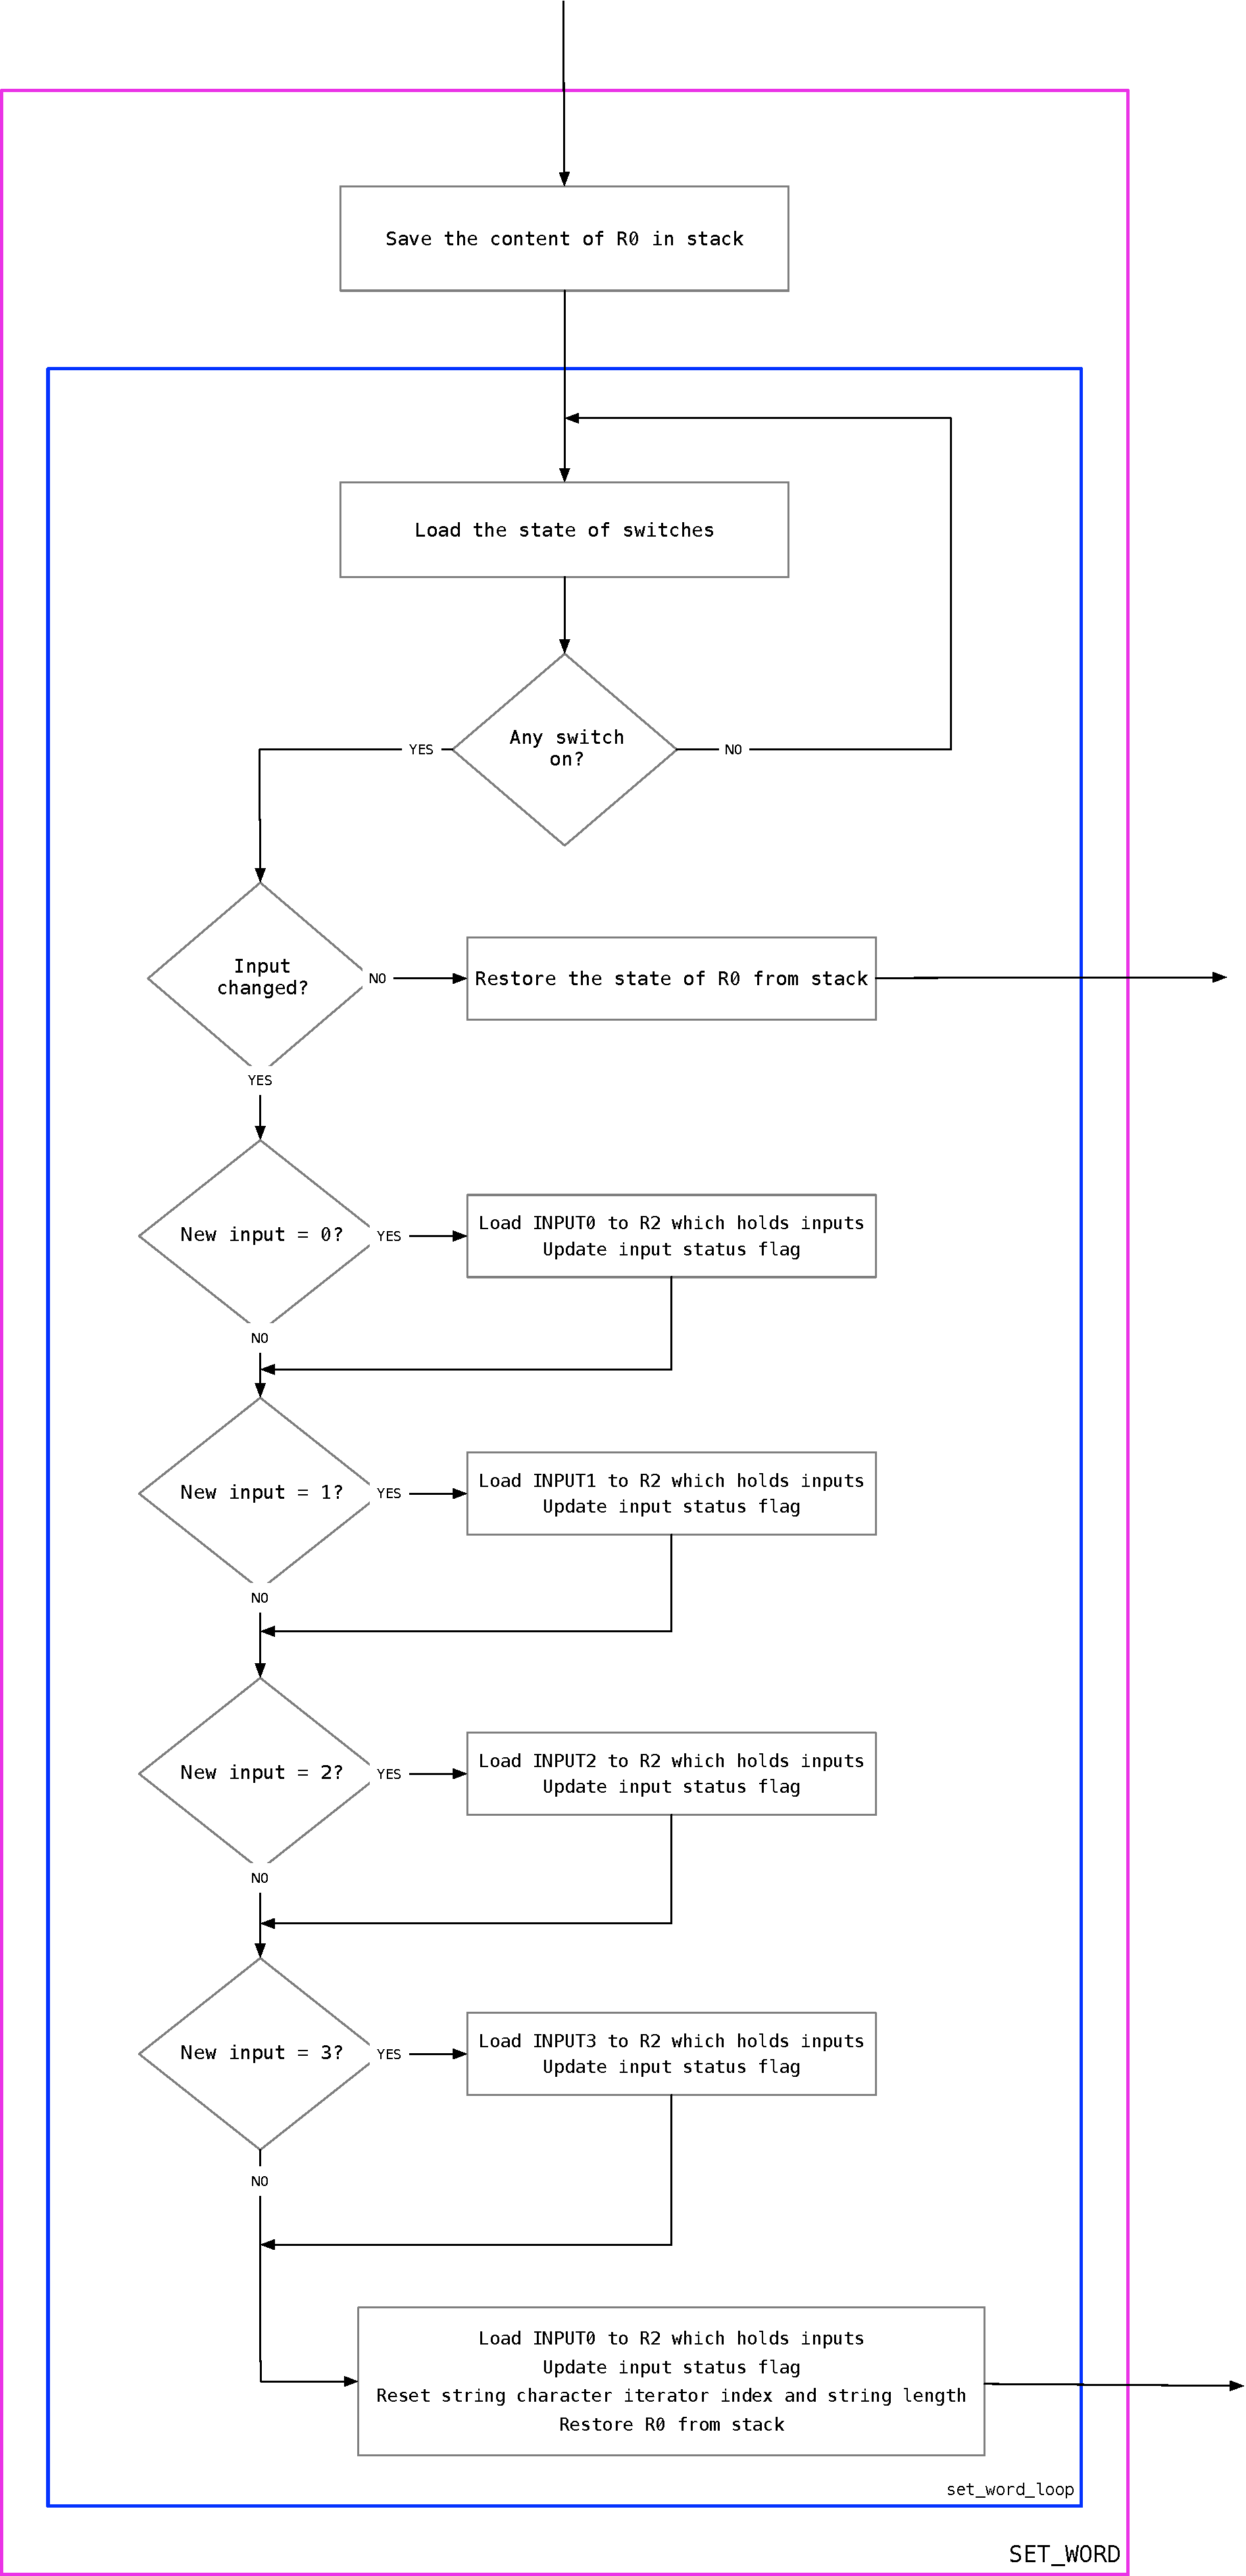
\includegraphics[scale=.25]{../images/set_word.pdf}
		\caption{Flowchart of Set Word Subroutine}
	\end{figure}
	\newpage
	\subsection{SET\_SPEED \& CHECK\_PAUSE}
	As the names suggests, \textit{SET\_SPEED} and \textit{CHECK\_PAUSE} subroutines are pausing the slider and sets its speed. Both of these functions are triggered by certain combinations of push buttons. They check the latest push button configuration pause or increase/decrease the speed accordingly. There are 3 different predefined levels of speed;
	\begin{itemize}
		\item Normal: 1 sec
		\item Fast: .25 sec
		\item Slow: 4 sec
	\end{itemize}
	\begin{figure}[h]
		\begin{minipage}{0.45\textwidth}
			\centering
			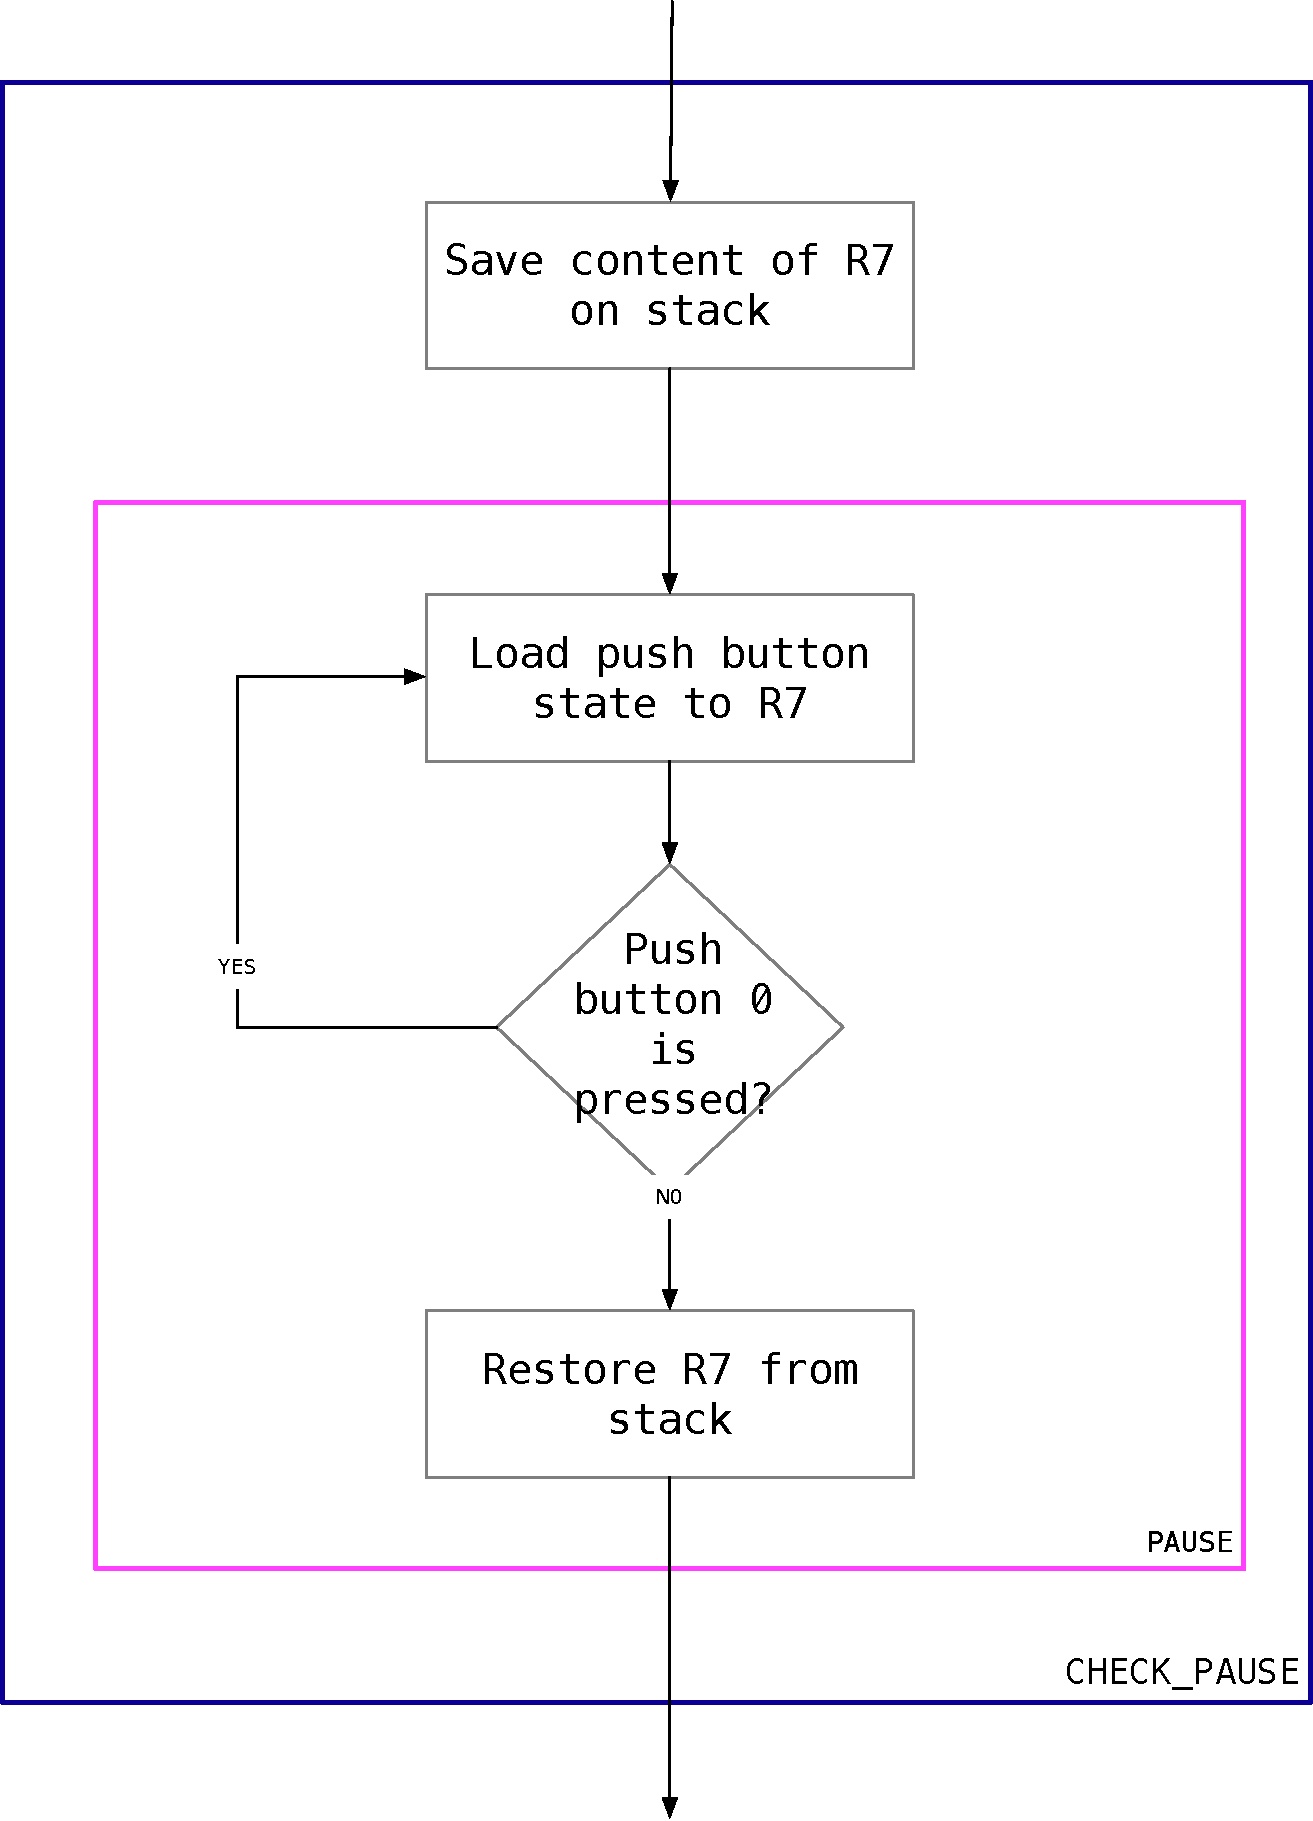
\includegraphics[scale=.3]{../images/check_pause.pdf}
			\caption{Flowchart of Check Pause Subroutine}
		\end{minipage}
		\begin{minipage}{0.7\linewidth}
			\centering
			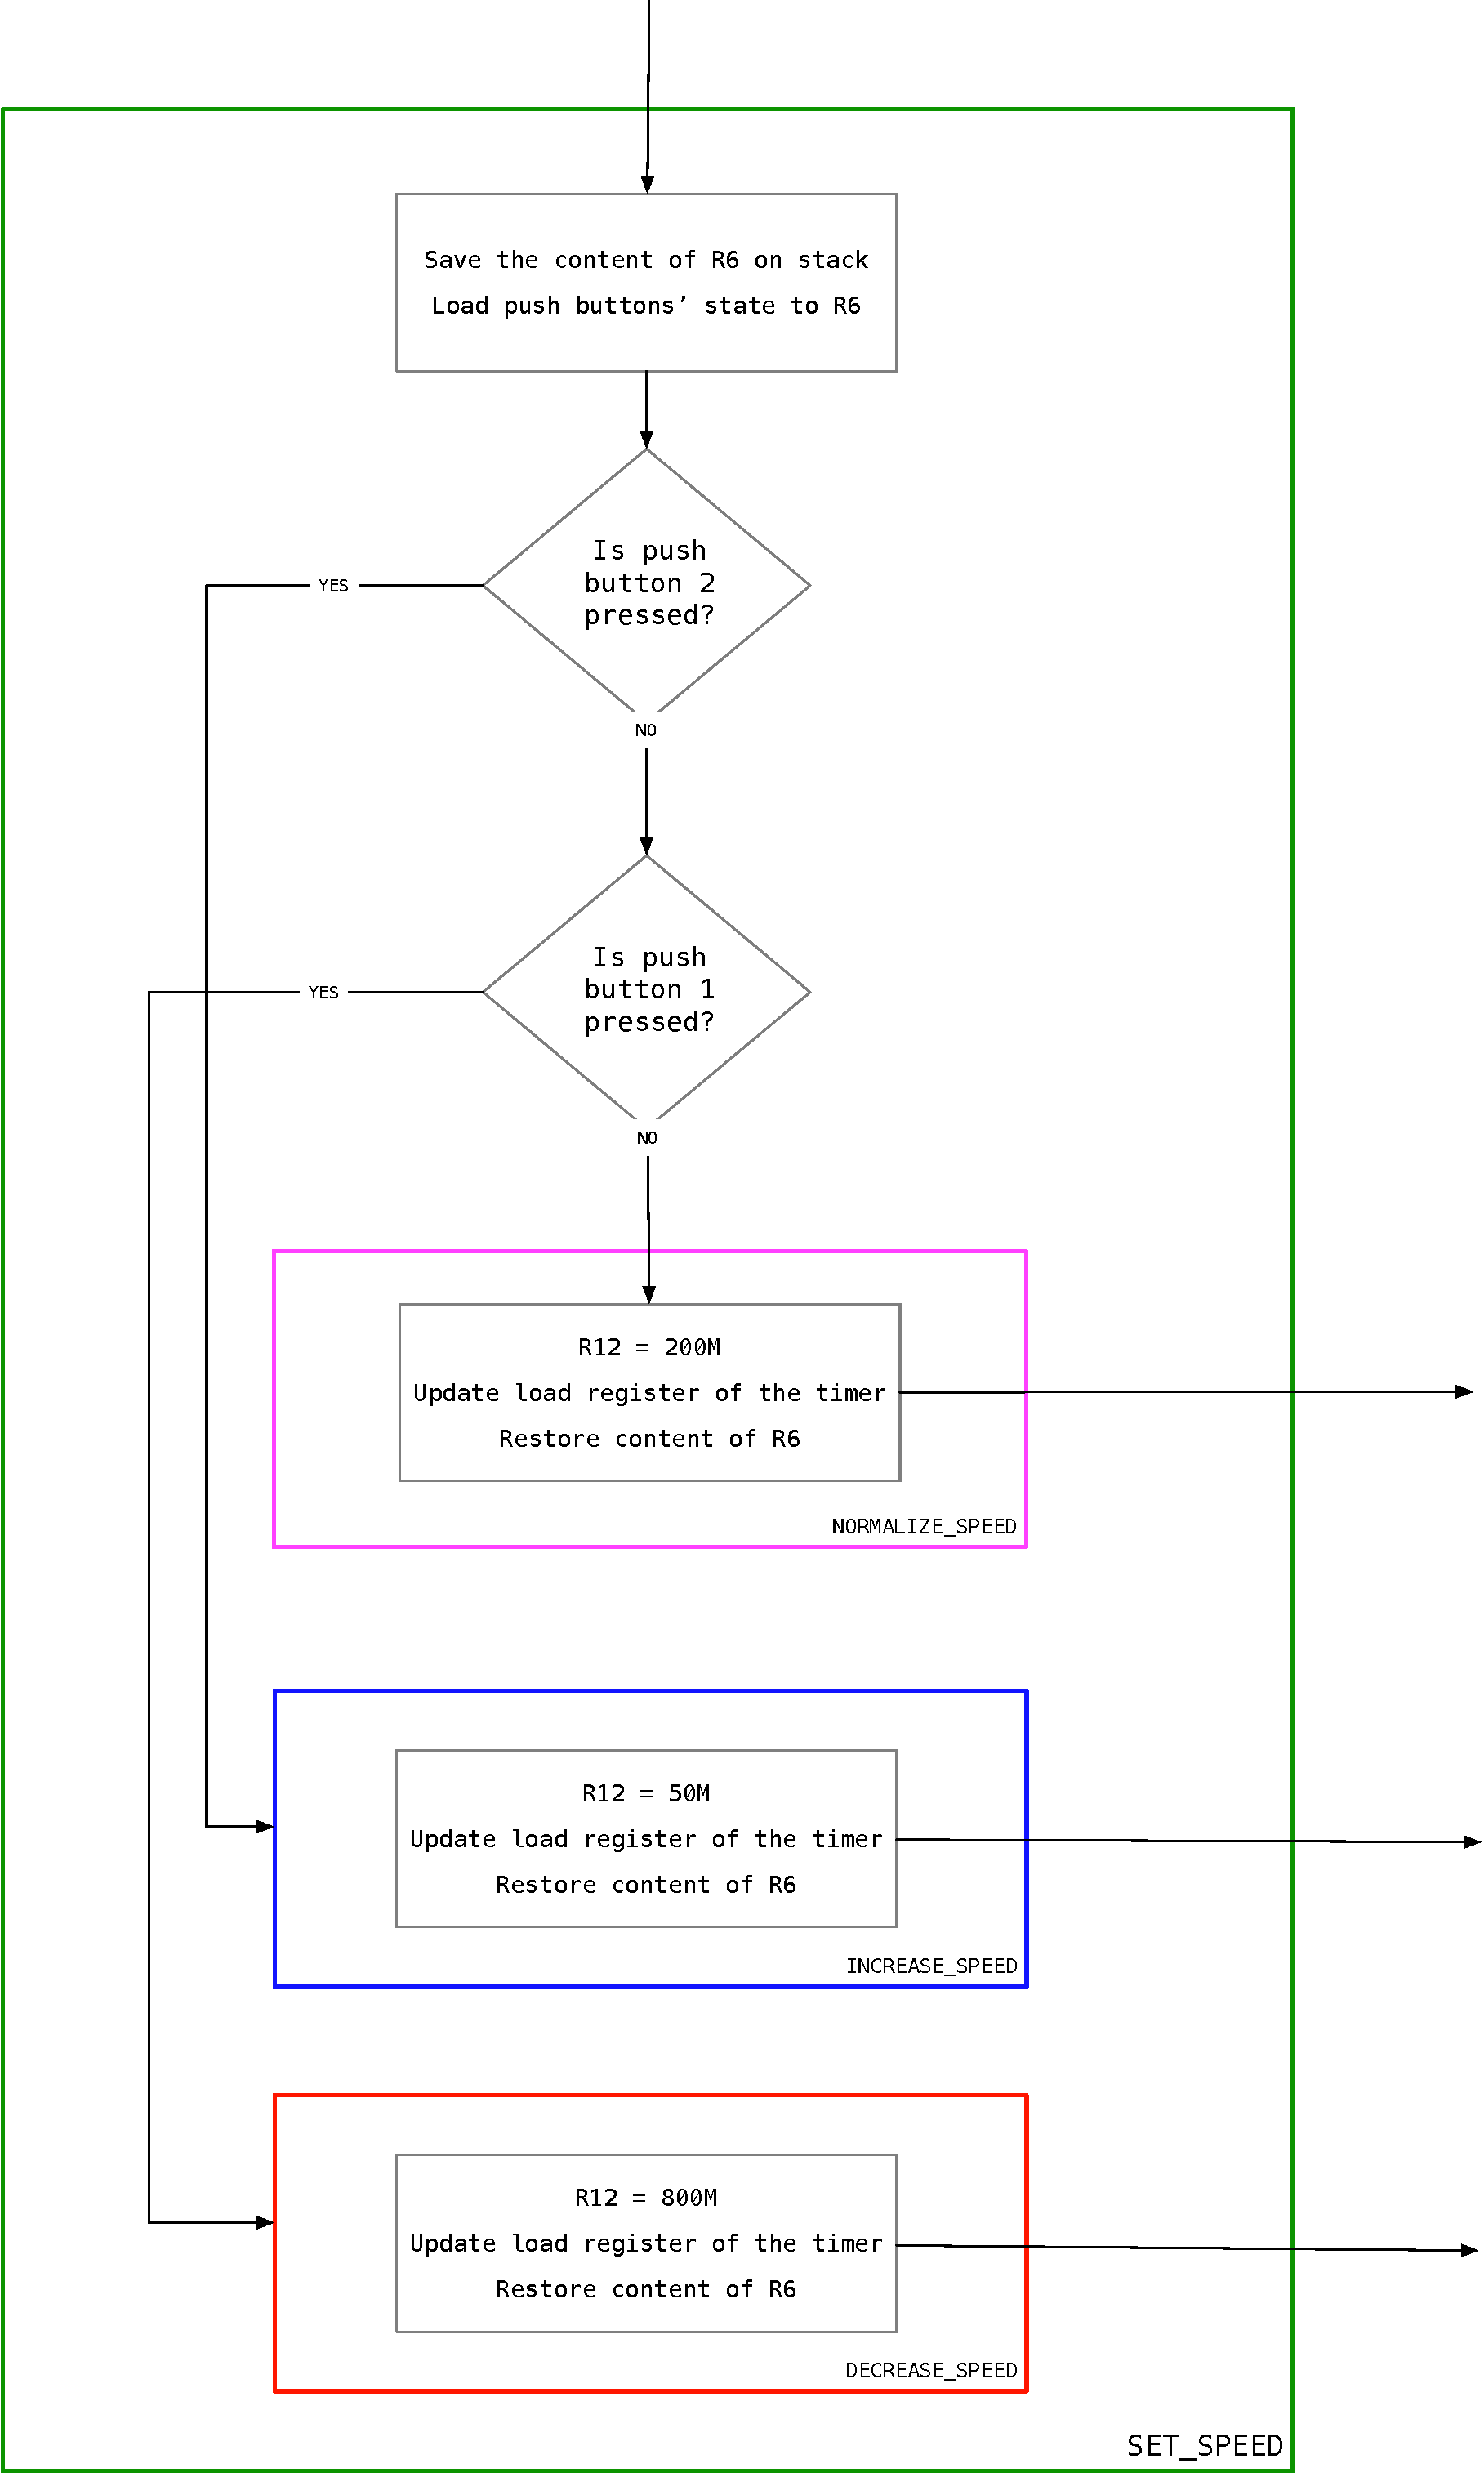
\includegraphics[scale=.3]{../images/set_speed.pdf}
			\caption{Flowchart of Set Speed Subroutine}
		\end{minipage}
	\end{figure}
	\newpage
	\subsection{PRINT\_STRING \& DELAY \& FIND\_LOC}
	\subsubsection{DELAY}
	The A9 Private Timer is being used for delays. This subroutine checks the timer configuration continuously until it finishes its countdown, after it finished this subroutine resets it and start over again when called next time.
	\subsubsection{PRINT\_STRING}
	This subroutine determines which letter to print relying on the input and which 7segment to print it.
	\subsubsection{FIND\_LOC}
	The representation of possible inputs, which are capital and lowercase letters along with numbers, are stored sequentially in the memory. This subroutine is used for locating the correct 7-segment representation in the memory.
	\begin{figure}[h]
		\centering
		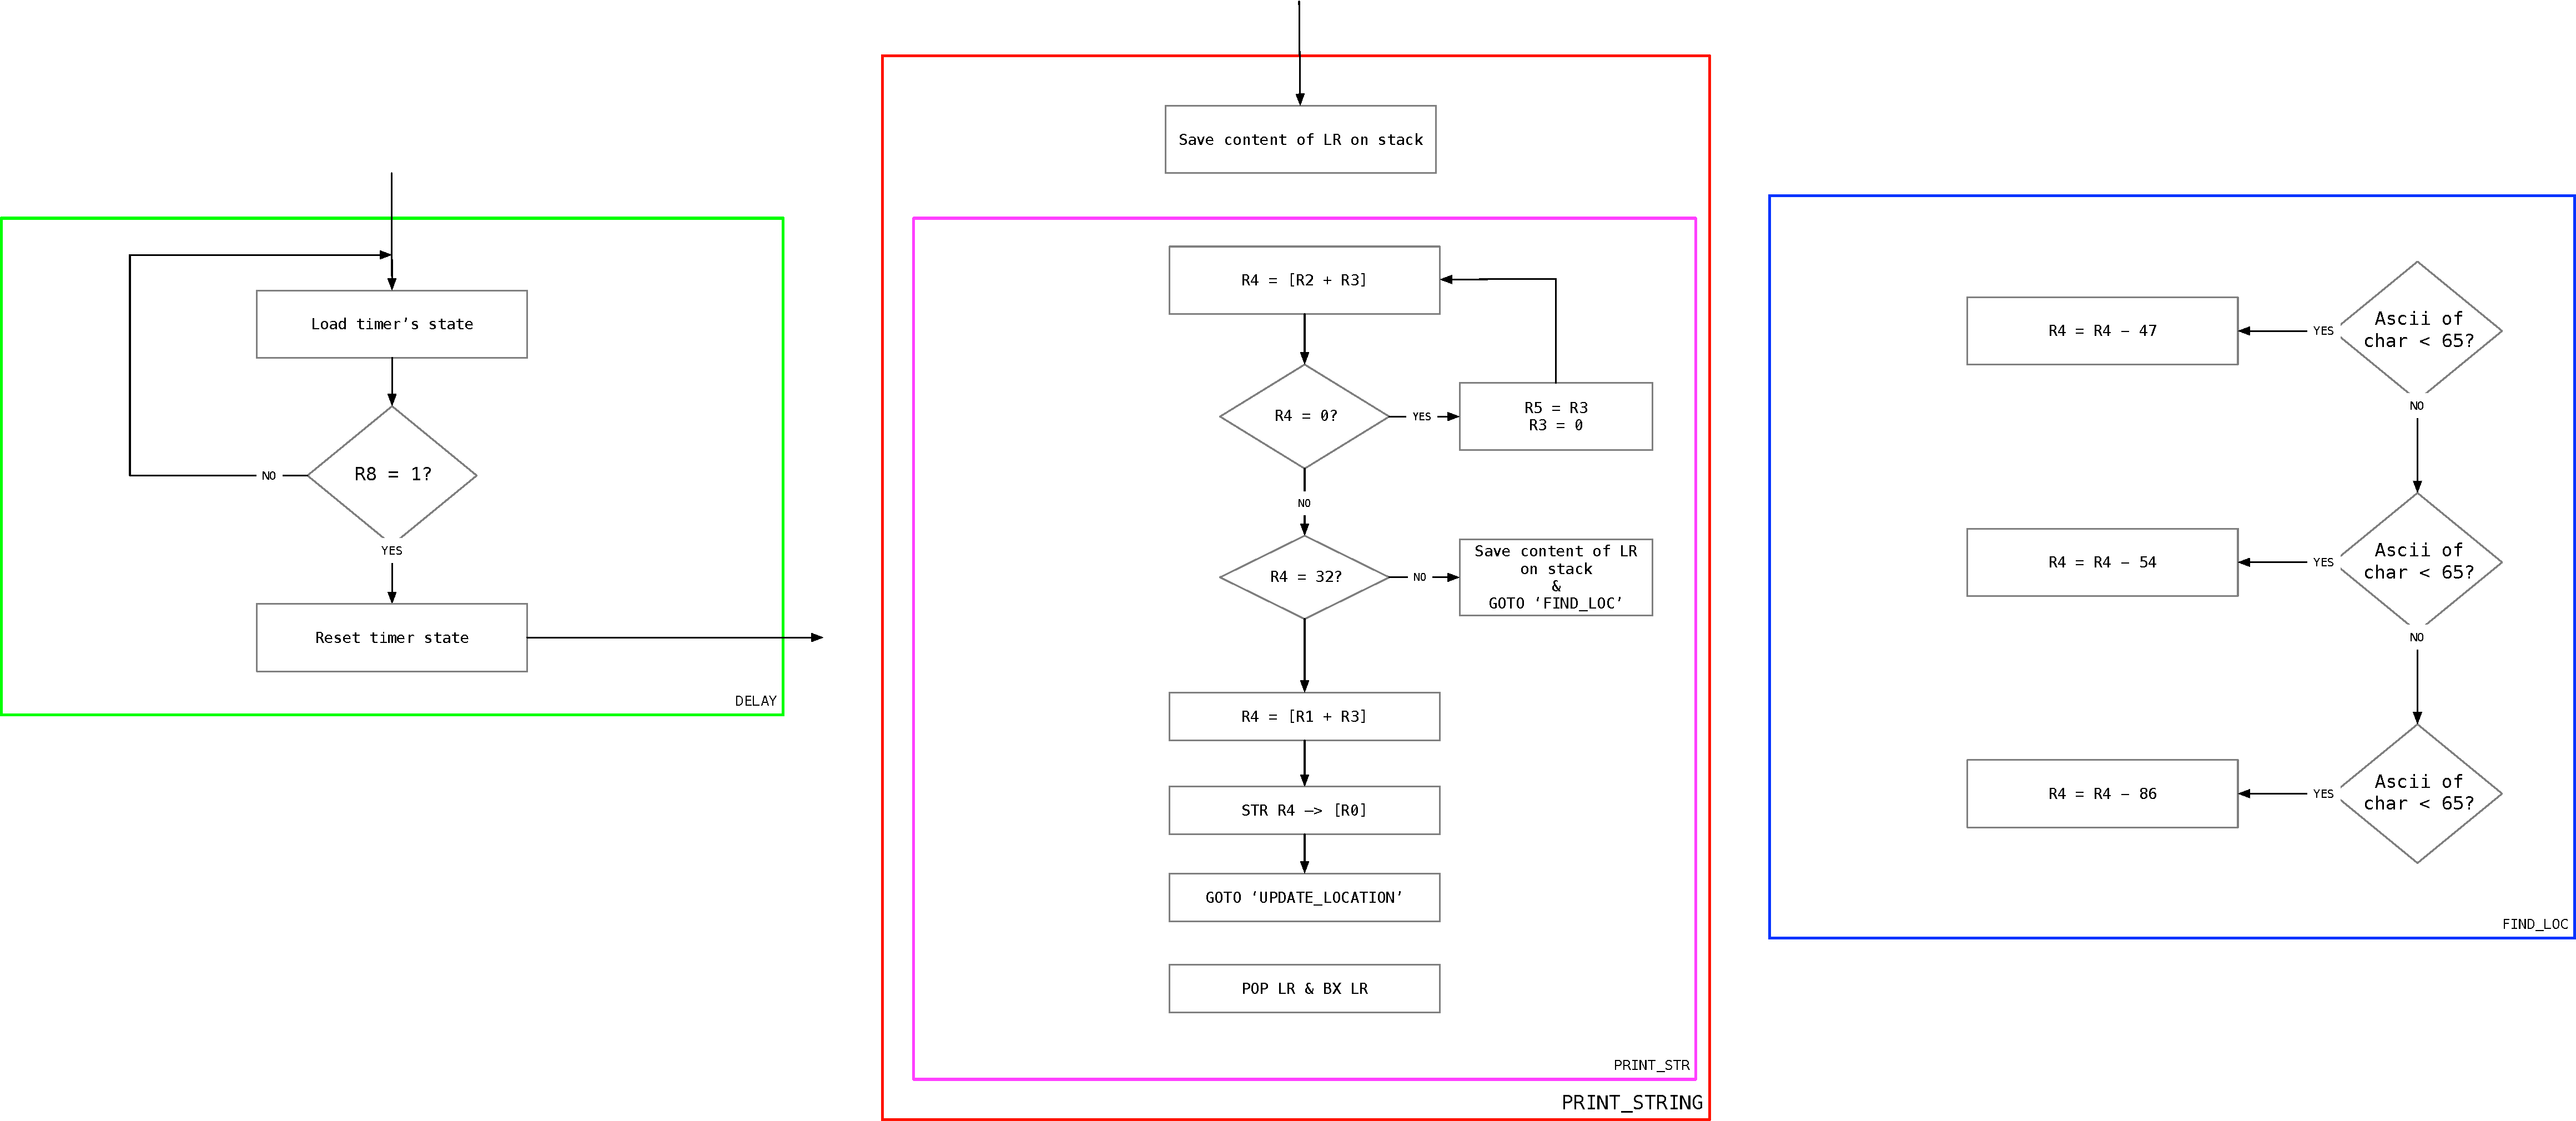
\includegraphics[scale=.15]{../images/print_string.pdf}
		\caption{Flowchart of Print String Method}
	\end{figure}
	\subsubsection{UPDATE\_LOCATION}
	\begin{wrapfigure}{r}{0.4\textwidth}
		\centering
		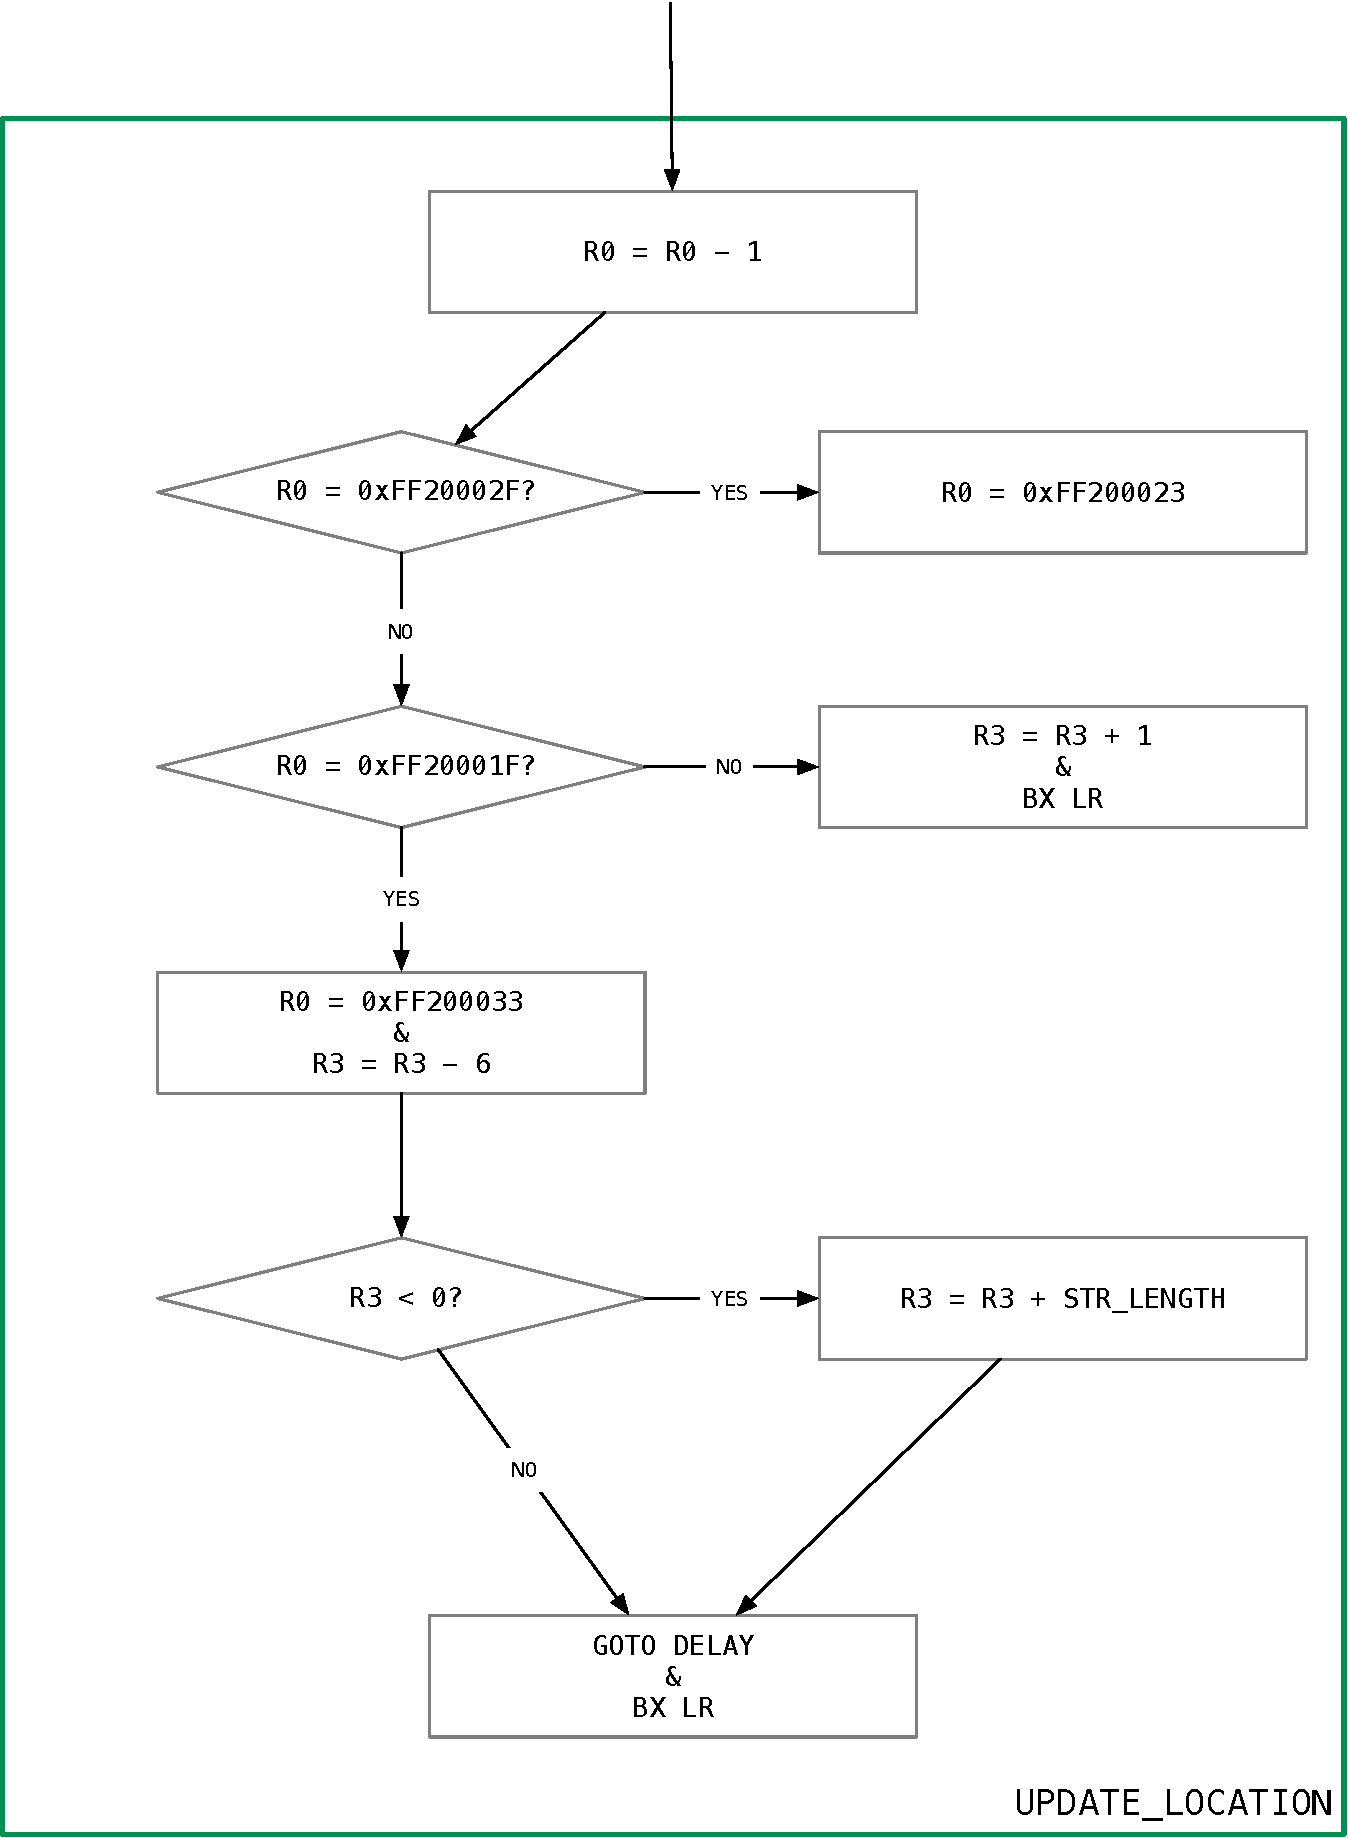
\includegraphics[scale=.2]{../images/update_location.pdf}
		\caption{Birds}
	\end{wrapfigure}
	This subroutine determines which 7-segment to write next character. Given that there are jumps between memory locations of 7-segments and circular loop, it has been decided that its best to handle these operations in a different subroutine. First we set it to be the 7-segment that is right next to the previous one. Then we check if has exceeded any limits, if it did, reset the position accordingly.



\end{document}